%%%%%%%%%%%%%%%%%%%%%%%%%%%%%%%%%%%%%%%%%
% The Legrand Orange Book
% LaTeX Template
% Version 2.1.1 (14/2/16)
%
% This template has been downloaded from:
% http://www.LaTeXTemplates.com
%
% Original author:
% Mathias Legrand (legrand.mathias@gmail.com) with modifications by:
% Vel (vel@latextemplates.com)
%
% License:
% CC BY-NC-SA 3.0 (http://creativecommons.org/licenses/by-nc-sa/3.0/)
%
% Compiling this template:
% This template uses biber for its bibliography and makeindex for its index.
% When you first open the template, compile it from the command line with the 
% commands below to make sure your LaTeX distribution is configured correctly:
%
% 1) pdflatex main
% 2) makeindex main.idx -s StyleInd.ist
% 3) biber main
% 4) pdflatex main x 2
%
% After this, when you wish to update the bibliography/index use the appropriate
% command above and make sure to compile with pdflatex several times 
% afterwards to propagate your changes to the document.
%
% This template also uses a number of packages which may need to be
% updated to the newest versions for the template to compile. It is strongly\\
% recommended you update your LaTeX distribution if you have any
% compilation errors.
%
% Important note:
% Chapter heading images should have a 2:1 width:height ratio,
% e.g. 920px width and 460px height.
%
%%%%%%%%%%%%%%%%%%%%%%%%%%%%%%%%%%%%%%%%%

%----------------------------------------------------------------------------------------
%	PACKAGES AND OTHER DOCUMENT CONFIGURATIONS
%----------------------------------------------------------------------------------------

\documentclass[12pt,fleqn,a4paper]{book} % Default font size and left-justified equations


%----------------------------------------------------------------------------------------

%%%%%%%%%%%%%%%%%%%%%%%%%%%%%%%%%%%%%%%%%
% The Legrand Orange Book
% Structural Definitions File
% Version 2.0 (9/2/15)
%
% Original author:
% Mathias Legrand (legrand.mathias@gmail.com) with modifications by:
% Vel (vel@latextemplates.com)
% 
% This file has been downloaded from:
% http://www.LaTeXTemplates.com
%
% License:
% CC BY-NC-SA 3.0 (http://creativecommons.org/licenses/by-nc-sa/3.0/)
%
%%%%%%%%%%%%%%%%%%%%%%%%%%%%%%%%%%%%%%%%%

%----------------------------------------------------------------------------------------
%	VARIOUS REQUIRED PACKAGES AND CONFIGURATIONS
%----------------------------------------------------------------------------------------

\usepackage[top=3cm,bottom=3cm,left=3cm,right=3cm,headsep=10pt,a4paper]{geometry} % Page margins
%\usepackage[top=1.5cm,bottom=1.5cm,left=2cm,right=1.5cm,headsep=10pt,a5paper]{geometry} % Page margins

\usepackage{graphicx} % Required for including pictures
\graphicspath{{Pictures/}} % Specifies the directory where pictures are stored

\usepackage{lipsum} % Inserts dummy text

\usepackage{tikz} % Required for drawing custom shapes

%\usepackage[english]{babel} % English language/hyphenation

\usepackage[italian]{babel}
\selectlanguage{italian}
\usepackage[T1]{fontenc}

%Overleaf
\usepackage[utf8]{inputenc}


\usepackage{enumitem} % Customize lists
\setlist{nolistsep} % Reduce spacing between bullet points and numbered lists

\usepackage{booktabs} % Required for nicer horizontal rules in tables

\usepackage{xcolor} % Required for specifying colors by name
\definecolor{ocre}{RGB}{243,102,25} % Define the orange color used for highlighting throughout the book

%----------------------------------------------------------------------------------------
%	FONTS
%----------------------------------------------------------------------------------------

\usepackage{avant} % Use the Avantgarde font for headings
%\usepackage{times} % Use the Times font for headings
\usepackage{mathptmx} % Use the Adobe Times Roman as the default text font together with math symbols from the Sym­bol, Chancery and Com­puter Modern fonts

\usepackage{microtype} % Slightly tweak font spacing for aesthetics
\usepackage[utf8]{inputenc} % Required for including letters with accents
\usepackage[T1]{fontenc} % Use 8-bit encoding that has 256 glyphs

%----------------------------------------------------------------------------------------
%	BIBLIOGRAPHY AND INDEX
%----------------------------------------------------------------------------------------

\usepackage{csquotes}
\usepackage[style=alphabetic,citestyle=numeric,sorting=nyt,sortcites=true,autopunct=true,autolang=hyphen,hyperref=true,abbreviate=false,backref=true,backend=biber,defernumbers=true]{biblatex}
\addbibresource{bibliography.bib} % BibTeX bibliography file
\defbibheading{bibempty}{}

\usepackage{calc} % For simpler calculation - used for spacing the index letter headings correctly
\usepackage{makeidx} % Required to make an index
\makeindex % Tells LaTeX to create the files required for indexing

%----------------------------------------------------------------------------------------
%	MAIN TABLE OF CONTENTS
%----------------------------------------------------------------------------------------

\usepackage{titletoc} % Required for manipulating the table of contents

\contentsmargin{0cm} % Removes the default margin

% Part text styling
\titlecontents{part}[0cm]
{\addvspace{20pt}\centering\large\bfseries}
{}
{}
{}

% Chapter text styling
\titlecontents{chapter}[1.25cm] % Indentation
{\addvspace{12pt}\large\sffamily\bfseries} % Spacing and font options for chapters
{\color{ocre!60}\contentslabel[\Large\thecontentslabel]{1.25cm}\color{ocre}} % Chapter number
{\color{ocre}}  
{\color{ocre!60}\normalsize\;\titlerule*[.5pc]{.}\;\thecontentspage} % Page number

% Section text styling
\titlecontents{section}[1.25cm] % Indentation
{\addvspace{3pt}\sffamily\bfseries} % Spacing and font options for sections
{\contentslabel[\thecontentslabel]{1.25cm}} % Section number
{}
{\hfill\color{black}\thecontentspage} % Page number
[]

% Subsection text styling
\titlecontents{subsection}[1.25cm] % Indentation
{\addvspace{1pt}\sffamily\small} % Spacing and font options for subsections
{\contentslabel[\thecontentslabel]{1.25cm}} % Subsection number
{}
{\ \titlerule*[.5pc]{.}\;\thecontentspage} % Page number
[]

% List of figures
\titlecontents{figure}[0em]
{\addvspace{-5pt}\sffamily}
{\thecontentslabel\hspace*{1em}}
{}
{\ \titlerule*[.5pc]{.}\;\thecontentspage}
[]

% List of tables
\titlecontents{table}[0em]
{\addvspace{-5pt}\sffamily}
{\thecontentslabel\hspace*{1em}}
{}
{\ \titlerule*[.5pc]{.}\;\thecontentspage}
[]

%----------------------------------------------------------------------------------------
%	MINI TABLE OF CONTENTS IN PART HEADS
%----------------------------------------------------------------------------------------

% Chapter text styling
\titlecontents{lchapter}[0em] % Indenting
{\addvspace{15pt}\large\sffamily\bfseries} % Spacing and font options for chapters
{\color{ocre}\contentslabel[\Large\thecontentslabel]{1.25cm}\color{ocre}} % Chapter number
{}  
{\color{ocre}\normalsize\sffamily\bfseries\;\titlerule*[.5pc]{.}\;\thecontentspage} % Page number

% Section text styling
\titlecontents{lsection}[0em] % Indenting
{\sffamily\small} % Spacing and font options for sections
{\contentslabel[\thecontentslabel]{1.25cm}} % Section number
{}
{}

% Subsection text styling
\titlecontents{lsubsection}[.5em] % Indentation
{\normalfont\footnotesize\sffamily} % Font settings
{}
{}
{}

%----------------------------------------------------------------------------------------
%	PAGE HEADERS
%----------------------------------------------------------------------------------------

\usepackage{fancyhdr} % Required for header and footer configuration

\pagestyle{fancy}
\renewcommand{\chaptermark}[1]{\markboth{\sffamily\normalsize\bfseries\chaptername\ \thechapter.\ #1}{}} % Chapter text font settings
\renewcommand{\sectionmark}[1]{\markright{\sffamily\normalsize\thesection\hspace{5pt}#1}{}} % Section text font settings
\fancyhf{} \fancyhead[LE,RO]{\sffamily\normalsize\thepage} % Font setting for the page number in the header
\fancyhead[LO]{\rightmark} % Print the nearest section name on the left side of odd pages
\fancyhead[RE]{\leftmark} % Print the current chapter name on the right side of even pages
\renewcommand{\headrulewidth}{0.5pt} % Width of the rule under the header
\addtolength{\headheight}{2.5pt} % Increase the spacing around the header slightly
\renewcommand{\footrulewidth}{0pt} % Removes the rule in the footer
\fancypagestyle{plain}{\fancyhead{}\renewcommand{\headrulewidth}{0pt}} % Style for when a plain pagestyle is specified

% Removes the header from odd empty pages at the end of chapters
\makeatletter
\renewcommand{\cleardoublepage}{
\clearpage\ifodd\c@page\else
\hbox{}
\vspace*{\fill}
\thispagestyle{empty}
\newpage
\fi}

%----------------------------------------------------------------------------------------
%	THEOREM STYLES
%----------------------------------------------------------------------------------------

\usepackage{amsmath,amsfonts,amssymb,amsthm} % For math equations, theorems, symbols, etc

\newcommand{\intoo}[2]{\mathopen{]}#1\,;#2\mathclose{[}}
\newcommand{\ud}{\mathop{\mathrm{{}d}}\mathopen{}}
\newcommand{\intff}[2]{\mathopen{[}#1\,;#2\mathclose{]}}
\newtheorem{notation}{Notation}[chapter]

% Boxed/framed environments
\newtheoremstyle{ocrenumbox}% % Theorem style name
{0pt}% Space above
{0pt}% Space below
{\normalfont}% % Body font
{}% Indent amount
{\small\bf\sffamily\color{ocre}}% % Theorem head font
{\;}% Punctuation after theorem head
{0.25em}% Space after theorem head
{\small\sffamily\color{ocre}\thmname{#1}\nobreakspace\thmnumber{\@ifnotempty{#1}{}\@upn{#2}}% Theorem text (e.g. Theorem 2.1)
\thmnote{\nobreakspace\the\thm@notefont\sffamily\bfseries\color{black}---\nobreakspace#3.}} % Optional theorem note
\renewcommand{\qedsymbol}{$\blacksquare$}% Optional qed square

\newtheoremstyle{blacknumex}% Theorem style name
{5pt}% Space above
{5pt}% Space below
{\normalfont}% Body font
{} % Indent amount
{\small\bf\sffamily}% Theorem head font
{\;}% Punctuation after theorem head
{0.25em}% Space after theorem head
{\small\sffamily{\tiny\ensuremath{\blacksquare}}\nobreakspace\thmname{#1}\nobreakspace\thmnumber{\@ifnotempty{#1}{}\@upn{#2}}% Theorem text (e.g. Theorem 2.1)
\thmnote{\nobreakspace\the\thm@notefont\sffamily\bfseries---\nobreakspace#3.}}% Optional theorem note

\newtheoremstyle{blacknumbox} % Theorem style name
{0pt}% Space above
{0pt}% Space below
{\normalfont}% Body font
{}% Indent amount
{\small\bf\sffamily}% Theorem head font
{\;}% Punctuation after theorem head
{0.25em}% Space after theorem head
{\small\sffamily\thmname{#1}\nobreakspace\thmnumber{\@ifnotempty{#1}{}\@upn{#2}}% Theorem text (e.g. Theorem 2.1)
\thmnote{\nobreakspace\the\thm@notefont\sffamily\bfseries---\nobreakspace#3.}}% Optional theorem note

% Non-boxed/non-framed environments
\newtheoremstyle{ocrenum}% % Theorem style name
{5pt}% Space above
{5pt}% Space below
{\normalfont}% % Body font
{}% Indent amount
{\small\bf\sffamily\color{ocre}}% % Theorem head font
{\;}% Punctuation after theorem head
{0.25em}% Space after theorem head
{\small\sffamily\color{ocre}\thmname{#1}\nobreakspace\thmnumber{\@ifnotempty{#1}{}\@upn{#2}}% Theorem text (e.g. Theorem 2.1)
\thmnote{\nobreakspace\the\thm@notefont\sffamily\bfseries\color{black}---\nobreakspace#3.}} % Optional theorem note
\renewcommand{\qedsymbol}{$\blacksquare$}% Optional qed square
\makeatother

% Defines the theorem text style for each type of theorem to one of the three styles above
\newcounter{dummy} 
\numberwithin{dummy}{section}
\theoremstyle{ocrenumbox}
\newtheorem{theoremeT}[dummy]{Teorema}
\newtheorem{problem}{Problema}[chapter]
\newtheorem{exerciseT}{Esercizio}[chapter]
\theoremstyle{blacknumex}
\newtheorem{exampleT}{Esempio}[chapter]
\theoremstyle{blacknumbox}
\newtheorem{vocabulary}{Vocabolario}[chapter]
\newtheorem{definitionT}{Definizione}[section]
\newtheorem{corollaryT}[dummy]{Corollario}
\theoremstyle{ocrenum}
\newtheorem{proposition}[dummy]{Proposizione}

%----------------------------------------------------------------------------------------
%	DEFINITION OF COLORED BOXES
%----------------------------------------------------------------------------------------

\RequirePackage[framemethod=default]{mdframed} % Required for creating the theorem, definition, exercise and corollary boxes

% Theorem box
\newmdenv[skipabove=7pt,
skipbelow=7pt,
backgroundcolor=black!5,
linecolor=ocre,
innerleftmargin=5pt,
innerrightmargin=5pt,
innertopmargin=5pt,
leftmargin=0cm,
rightmargin=0cm,
innerbottommargin=5pt]{tBox}

% Exercise box	  
\newmdenv[skipabove=7pt,
skipbelow=7pt,
rightline=false,
leftline=true,
topline=false,
bottomline=false,
backgroundcolor=ocre!10,
linecolor=ocre,
innerleftmargin=5pt,
innerrightmargin=5pt,
innertopmargin=5pt,
innerbottommargin=5pt,
leftmargin=0cm,
rightmargin=0cm,
linewidth=4pt]{eBox}	

% Definition box
\newmdenv[skipabove=7pt,
skipbelow=7pt,
rightline=false,
leftline=true,
topline=false,
bottomline=false,
linecolor=ocre,
innerleftmargin=5pt,
innerrightmargin=5pt,
innertopmargin=0pt,
leftmargin=0cm,
rightmargin=0cm,
linewidth=4pt,
innerbottommargin=0pt]{dBox}	

% Corollary box
\newmdenv[skipabove=7pt,
skipbelow=7pt,
rightline=false,
leftline=true,
topline=false,
bottomline=false,
linecolor=gray,
backgroundcolor=black!5,
innerleftmargin=5pt,
innerrightmargin=5pt,
innertopmargin=5pt,
leftmargin=0cm,
rightmargin=0cm,
linewidth=4pt,
innerbottommargin=5pt]{cBox}

% Creates an environment for each type of theorem and assigns it a theorem text style from the "Theorem Styles" section above and a colored box from above
\newenvironment{theorem}{\begin{tBox}\begin{theoremeT}}{\end{theoremeT}\end{tBox}}
\newenvironment{exercise}{\begin{eBox}\begin{exerciseT}}{\hfill{\color{ocre}\tiny\ensuremath{\blacksquare}}\end{exerciseT}\end{eBox}}				  
\newenvironment{definition}{\begin{dBox}\begin{definitionT}}{\end{definitionT}\end{dBox}}	
\newenvironment{example}{\begin{exampleT}}{\hfill{\tiny\ensuremath{\blacksquare}}\end{exampleT}}		
\newenvironment{corollary}{\begin{cBox}\begin{corollaryT}}{\end{corollaryT}\end{cBox}}	

%----------------------------------------------------------------------------------------
%	REMARK ENVIRONMENT
%----------------------------------------------------------------------------------------

\newenvironment{remark}{\par\vspace{10pt}\small % Vertical white space above the remark and smaller font size
\begin{list}{}{
\leftmargin=35pt % Indentation on the left
\rightmargin=25pt}\item\ignorespaces % Indentation on the right
\makebox[-2.5pt]{\begin{tikzpicture}[overlay]
\node[draw=ocre!60,line width=1pt,circle,fill=ocre!25,font=\sffamily\bfseries,inner sep=2pt,outer sep=0pt] at (-15pt,0pt){\textcolor{ocre}{R}};\end{tikzpicture}} % Orange R in a circle
\advance\baselineskip -1pt}{\end{list}\vskip5pt} % Tighter line spacing and white space after remark

%----------------------------------------------------------------------------------------
%	SECTION NUMBERING IN THE MARGIN
%----------------------------------------------------------------------------------------

\makeatletter
\renewcommand{\@seccntformat}[1]{\llap{\textcolor{ocre}{\csname the#1\endcsname}\hspace{1em}}}                    
\renewcommand{\section}{\@startsection{section}{1}{\z@}
{-4ex \@plus -1ex \@minus -.4ex}
{1ex \@plus.2ex }
{\normalfont\large\sffamily\bfseries}}
\renewcommand{\subsection}{\@startsection {subsection}{2}{\z@}
{-3ex \@plus -0.1ex \@minus -.4ex}
{0.5ex \@plus.2ex }
{\normalfont\sffamily\bfseries}}
\renewcommand{\subsubsection}{\@startsection {subsubsection}{3}{\z@}
{-2ex \@plus -0.1ex \@minus -.2ex}
{.2ex \@plus.2ex }
{\normalfont\small\sffamily\bfseries}}                        
\renewcommand\paragraph{\@startsection{paragraph}{4}{\z@}
{-2ex \@plus-.2ex \@minus .2ex}
{.1ex}
{\normalfont\small\sffamily\bfseries}}

%----------------------------------------------------------------------------------------
%	PART HEADINGS
%----------------------------------------------------------------------------------------

% numbered part in the table of contents
\newcommand{\@mypartnumtocformat}[2]{%
\setlength\fboxsep{0pt}%
\noindent\colorbox{ocre!20}{\strut\parbox[c][.7cm]{\ecart}{\color{ocre!70}\Large\sffamily\bfseries\centering#1}}\hskip\esp\colorbox{ocre!40}{\strut\parbox[c][.7cm]{\linewidth-\ecart-\esp}{\Large\sffamily\centering#2}}}%
%%%%%%%%%%%%%%%%%%%%%%%%%%%%%%%%%%
% unnumbered part in the table of contents
\newcommand{\@myparttocformat}[1]{%
\setlength\fboxsep{0pt}%
\noindent\colorbox{ocre!40}{\strut\parbox[c][.7cm]{\linewidth}{\Large\sffamily\centering#1}}}%
%%%%%%%%%%%%%%%%%%%%%%%%%%%%%%%%%%
\newlength\esp
\setlength\esp{4pt}
\newlength\ecart
\setlength\ecart{1.2cm-\esp}
\newcommand{\thepartimage}{}%
\newcommand{\partimage}[1]{\renewcommand{\thepartimage}{#1}}%
\def\@part[#1]#2{%
\ifnum \c@secnumdepth >-2\relax%
\refstepcounter{part}%
\addcontentsline{toc}{part}{\texorpdfstring{\protect\@mypartnumtocformat{\thepart}{#1}}{\partname~\thepart\ ---\ #1}}
\else%
\addcontentsline{toc}{part}{\texorpdfstring{\protect\@myparttocformat{#1}}{#1}}%
\fi%
\startcontents%
\markboth{}{}%
{\thispagestyle{empty}%
\begin{tikzpicture}[remember picture,overlay]%
\node at (current page.north west){\begin{tikzpicture}[remember picture,overlay]%	
\fill[ocre!20](0cm,0cm) rectangle (\paperwidth,-\paperheight);
\node[anchor=north] at (4cm,-3.25cm){\color{ocre!40}\fontsize{220}{100}\sffamily\bfseries\@Roman\c@part}; 
\node[anchor=south east] at (\paperwidth-1cm,-\paperheight+1cm){\parbox[t][][t]{8.5cm}{
\printcontents{l}{0}{\setcounter{tocdepth}{1}}%
}};
\node[anchor=north east] at (\paperwidth-1.5cm,-3.25cm){\parbox[t][][t]{15cm}{\strut\raggedleft\color{white}\fontsize{30}{30}\sffamily\bfseries#2}};
\end{tikzpicture}};
\end{tikzpicture}}%
\@endpart}
\def\@spart#1{%
\startcontents%
\phantomsection
{\thispagestyle{empty}%
\begin{tikzpicture}[remember picture,overlay]%
\node at (current page.north west){\begin{tikzpicture}[remember picture,overlay]%	
\fill[ocre!20](0cm,0cm) rectangle (\paperwidth,-\paperheight);
\node[anchor=north east] at (\paperwidth-1.5cm,-3.25cm){\parbox[t][][t]{15cm}{\strut\raggedleft\color{white}\fontsize{30}{30}\sffamily\bfseries#1}};
\end{tikzpicture}};
\end{tikzpicture}}
\addcontentsline{toc}{part}{\texorpdfstring{%
\setlength\fboxsep{0pt}%
\noindent\protect\colorbox{ocre!40}{\strut\protect\parbox[c][.7cm]{\linewidth}{\Large\sffamily\protect\centering #1\quad\mbox{}}}}{#1}}%
\@endpart}
\def\@endpart{\vfil\newpage
\if@twoside
\if@openright
\null
\thispagestyle{empty}%
\newpage
\fi
\fi
\if@tempswa
\twocolumn
\fi}

%----------------------------------------------------------------------------------------
%	CHAPTER HEADINGS
%----------------------------------------------------------------------------------------

% A switch to conditionally include a picture, implemented by  Christian Hupfer
\newif\ifusechapterimage
\usechapterimagetrue
\newcommand{\thechapterimage}{}%
\newcommand{\chapterimage}[1]{\ifusechapterimage\renewcommand{\thechapterimage}{#1}\fi}%
\def\@makechapterhead#1{%
{\parindent \z@ \raggedright \normalfont
\ifnum \c@secnumdepth >\m@ne
\if@mainmatter
\begin{tikzpicture}[remember picture,overlay]
\node at (current page.north west)
{\begin{tikzpicture}[remember picture,overlay]
\node[anchor=north west,inner sep=0pt] at (0,0) {\ifusechapterimage\includegraphics[width=\paperwidth]{\thechapterimage}\fi};
\draw[anchor=west] (\Gm@lmargin,-9cm) node [line width=2pt,rounded corners=15pt,draw=ocre,fill=white,fill opacity=0.5,inner sep=15pt]{\strut\makebox[22cm]{}};
\draw[anchor=west] (\Gm@lmargin+.3cm,-9cm) node {\huge\sffamily\bfseries\color{black}\thechapter. #1\strut};
\end{tikzpicture}};
\end{tikzpicture}
\else
\begin{tikzpicture}[remember picture,overlay]
\node at (current page.north west)
{\begin{tikzpicture}[remember picture,overlay]
\node[anchor=north west,inner sep=0pt] at (0,0) {\ifusechapterimage\includegraphics[width=\paperwidth]{\thechapterimage}\fi};
\draw[anchor=west] (\Gm@lmargin,-9cm) node [line width=2pt,rounded corners=15pt,draw=ocre,fill=white,fill opacity=0.5,inner sep=15pt]{\strut\makebox[22cm]{}};
\draw[anchor=west] (\Gm@lmargin+.3cm,-9cm) node {\huge\sffamily\bfseries\color{black}#1\strut};
\end{tikzpicture}};
\end{tikzpicture}
\fi\fi\par\vspace*{270\p@}}}

%-------------------------------------------

\def\@makeschapterhead#1{%
\begin{tikzpicture}[remember picture,overlay]
\node at (current page.north west)
{\begin{tikzpicture}[remember picture,overlay]
\node[anchor=north west,inner sep=0pt] at (0,0) {\ifusechapterimage\includegraphics[width=\paperwidth]{\thechapterimage}\fi};
\draw[anchor=west] (\Gm@lmargin,-9cm) node [line width=2pt,rounded corners=15pt,draw=ocre,fill=white,fill opacity=0.5,inner sep=15pt]{\strut\makebox[22cm]{}};
\draw[anchor=west] (\Gm@lmargin+.3cm,-9cm) node {\huge\sffamily\bfseries\color{black}#1\strut};
\end{tikzpicture}};
\end{tikzpicture}
\par\vspace*{270\p@}}
\makeatother

%----------------------------------------------------------------------------------------
%	HYPERLINKS IN THE DOCUMENTS
%----------------------------------------------------------------------------------------

\usepackage{hyperref}
\hypersetup{hidelinks,colorlinks=false,breaklinks=true,urlcolor= ocre,bookmarksopen=false,pdftitle={Title},pdfauthor={Author}}
\usepackage{bookmark}
\bookmarksetup{
open,
numbered,
addtohook={%
\ifnum\bookmarkget{level}=0 % chapter
\bookmarksetup{bold}%
\fi
\ifnum\bookmarkget{level}=-1 % part
\bookmarksetup{color=ocre,bold}%
\fi
}
}
 % Insert the commands.tex file which contains the majority of the structure behind the template

\usepackage{array}

    \begin{document}
    
    %----------------------------------------------------------------------------------------
    %	TITLE PAGE
    %----------------------------------------------------------------------------------------
    
    \begingroup
    \thispagestyle{empty}
    \begin{tikzpicture}[remember picture,overlay]
    \coordinate [below=12cm] (midpoint) at (current page.north);
    \node at (current page.north west)
    {\begin{tikzpicture}[remember picture,overlay]
    \node[anchor=north west,inner sep=0pt] at (0,0) {
\includegraphics[width=\paperwidth]{background}}; % Background image
    \draw[anchor=north] (midpoint) node [fill=ocre!30!white,fill opacity=0.6,text opacity=1,inner sep=1cm]{\Huge\centering\bfseries\sffamily\parbox[c][][t]{\paperwidth}{\centering Laboratorio di informatica\\[15pt] % Book title
    {\Large ~}\\[20pt] % Subtitle
    {\huge Dot. Ing. Matteo Ginesi}}}; % Author name
    \end{tikzpicture}};
    \end{tikzpicture}
    \vfill
    \endgroup
    
    %----------------------------------------------------------------------------------------
    %	COPYRIGHT PAGE
    %----------------------------------------------------------------------------------------
    
    \newpage
    \begin{quote}
    	\begin{flushright}
    		\footnotesize
    		\textit{
			Did you hear baby\\
			Come back and tell you the things he's seen.\\
			Did it surprise you\\
			To be picked up at eight in a limousine?\\
			Doing the things he's accustomed to do.\\
			Which at one time it seemed like a dream\\
			Now it's true.\\
			And unknowing\\
			You made it all happen this way.\\ ~ \\} 
			Jethro Tull - For a Thousand Mothers
    	\end{flushright}
    \end{quote}
    ~\vfill
    \thispagestyle{empty}
    
    \noindent Copyright \copyright\ 2019 Matteo Ginesi\\ % Copyright notice
 
 	\noindent Scritto da: Matteo Ginesi, 2019   
 	
%    \noindent \textsc{Published by Publisher}\\ % Publisher
    
    \noindent \url{https://github.com/matginesi/InfoLab}\\ % URL
    
    \begin{figure}[h!]
    	\centering
\includegraphics[scale=1]{Pictures/by-sa.png}
    \end{figure}
    
    \noindent This work is licensed under the Creative Commons Attribution-ShareAlike 4.0 International License. To view a copy of this license, visit http://creativecommons.org/licenses/by-sa/4.0/ or send a letter to Creative Commons, PO Box 1866, Mountain View, CA 94042, USA.\\
    
    \noindent \textit{Prima edizione, speriamo presto} % Printing/edition date
    
    %----------------------------------------------------------------------------------------
    %	TABLE OF CONTENTS
    %----------------------------------------------------------------------------------------
    
    %\usechapterimagefalse % If you don't want to include a chapter image, use this to toggle images off - it can be enabled later with \usechapterimagetrue
    
    \chapterimage{chapter_head_1.pdf} % Table of contents heading image
    
    \pagestyle{empty} % No headers
    
    \tableofcontents % Print the table of contents itself
    
    \cleardoublepage % Forces the first chapter to start on an odd page so it's on the right
    
    \pagestyle{fancy} % Print headers again
    
    %----------------------------------------------------------------------------------------
    %	PART
    %----------------------------------------------------------------------------------------
    
    \part{Classe quarta}
    \label{part: Classe quarta}
    
    %----------------------------------------------------------------------------------------
    %	CHAPTER 1
    %----------------------------------------------------------------------------------------
    
    \chapterimage{chapter_head_2.pdf} % Chapter heading image
    
    \chapter{Introduzione}
    \label{cap: Introduzione}
        
        \section{L'informatica}\index{L'informatica}
        \label{sec: L'informatica oggi}
    		Ognuno di noi ha avuto a che fare con l'informatica nella vita di tutti i giorni. Un esempio? Vi è mai squillato il telefono? Avete mai acceso una consolle per giocare? Avete mai utilizzato un computer? Avete mai visto un video su internet? Avete mai avuto in mano un tablet?\\ Se avete risposto "si" anche ad una sola delle domande, avete certamente avuto a che fare con l'informatica.
    		
    		Troppo spesso si associa la parola \textbf{informatica} alla parola \textbf{computer}: questo in parte è giusto, ma non del tutto: il computer è solo uno dei tanti sistemi informatici esistenti. L'informatica è una \textbf{scienza} e come tale si occupa di molte cose.
    		A proposito di computer, questa è la definizione presa dall'enciclopedia (che termine antico!) \textit{online} per eccellenza, ovvero \textit{Wikipedia}\footnote{Sito web: \url{https://www.wikipedia.org}}, della parola \textbf{informatica}\footnote{Sito web: \url{https://it.wikipedia.org/wiki/Informatica}}:    		
    		\begin{definition}[Informatica]\label{def: Informatica}
    			\textit{L'informatica è la scienza che si occupa del trattamento dell'informazione mediante procedure automatizzate. In particolare ha per oggetto lo studio dei fondamenti teorici dell'informazione, della sua computazione a livello logico e delle tecniche pratiche per la sua implementazione e applicazione in sistemi elettronici automatizzati detti quindi sistemi informatici. Come tale è una disciplina fortemente connessa con l'automatica, l'elettronica e anche l'elettromeccanica.}
    		\end{definition}
    	
    		Non vi allarmate! Capisco che questa definizione possa sembrare davvero difficile, spesso incomprensibile, ma vi assicuro che non c'è altro di più facile: sono solo paroloni di addetti ai lavori... Analizziamo insieme tutte le parole \textit{difficili} e diamo un senso alla definizione.
    	
    		\subsection{L'informazione}\index{L'informazione}
    		\label{sub: L'informazione}
    			Notiamo subito che la definizione parla di \textit{trattamento delle informazioni}, ma cosa è un'\textbf{informazione}\footnote{Sito web: \url{http://www.treccani.it/enciclopedia/informazione/}}?
    			\begin{definition}[Informazione]\label{def: Informazione}
    				\textit{Notizia, dato o elemento che consente di avere conoscenza più o meno esatta di fatti, situazioni, modi di essere. In senso più generale, anche la trasmissione dei dati e l’insieme delle strutture che la consentono.}
    			\end{definition}
    		
				Possiamo dunque dire che un'\textbf{informazione} è una qualsiasi cosa ci fornisce più \textit{conoscenza} su un determinato argomento, situazione o momento. Conoscere è alla base della nostra società (ma vi posso garantire che è anche  alla base \textit{dell'universo, la vita e tutto quanto}\footnote{Squisita citazione da: \textit{Guida galattica per autostoppisti} - D. Adams. Gran bel libro.}). Siamo alla costante ricerca di \textbf{informazioni}, ad esempio:
    			\begin{itemize}
    				\item A che ora finisce la lezione?
    				\item A che ora inizia la ricreazione?
    				\item Quando è pronto il pranzo?
    				\item Quando sono nato?
    				\item Cosa è questo?
    				\item Come si chiama il compagno di classe?
    			\end{itemize}
    			Queste ed altre \textbf{domande} ce le poniamo fin da quando siamo bambini (soprattutto quella del pranzo...); infatti, fin da neonati abbiamo cominciato a collezionare \textbf{informazioni} utili per la nostra sopravvivenza: non ve ne siete mai accorti? Beh... chiedetevi come avete fatto ad imparare a chiamare i vostri genitori, i vostri amici. Chiedetevi come è possibile che quello strano sentimento allo stomaco, che chiamiamo \textit{fame}, significa "è l'ora di mangiare qualcosa!". Chi ve lo ha insegnato? La risposta è semplice: nessuno. Lo avete imparato da soli, proprio \textbf{collezionando informazioni intorno a voi}. Strana la vita eh?
    			\begin{exercise}
    				Cosa è un'informazione?
    			\end{exercise}    		
    			\begin{exercise}
    				Come possiamo ricavare un'informazione?
    			\end{exercise}
    			
    		\subsection{Automazione}\index{Automazione}
    		\label{sub: Automazione}
    			Andando avanti con la lettura della definizione di informatica (\ref{def: Informatica}, pag. \pageref{def: Informatica}), troviamo la frase "mediante procedure \textbf{automatizzate}". Cosa è l'automazione? Partiamo dalla definizione di \textbf{automatico}\footnote{Sito web: \url{http://www.treccani.it/vocabolario/automatico/}}:
    			\begin{definition}[Automatico]\label{def: Automatico}
    				\textit{Macchina, meccanismo o dispositivo che, regolato opportunamente, è capace di compiere determinate operazioni o lavorazioni, [...] senza il diretto intervento dell'uomo.}
    			\end{definition}
    		
    			Sicuramente tutti staranno già pensando "\textit{Ma che bella l'ora di informatica!}" (si, ne sono certo!), quindi voglio farvi un esempio semplice, banale ed anche divertente di sistema automatico: \textbf{lo sciacquone del gabinetto}. Tramite un piccolo gesto, l'acqua scorre nella tazza mandando via tutto ciò che c'era dentro. Senza l'aiuto di nessuno, nuova acqua scorre nel suo contenitore apposito ed è pronta per un nuovo utilizzo (ad esempio se non si è finito ciò che si era appena fatto, o se il precedente lavoro di arte moderna non è andato del tutto via!).
    			Per quanto mi riguarda, lo sciacquone, è il mio esempio preferito di sistema automatico.
    			
    			Altri esempi nella vita di tutti i giorni sono: l'ascensore, il distributore di merendine, il citofono... tutti molto utili, molto "raffinati", ben "ingegnerizzati", ma comunque non molto diversi dal nostro caro sciacquone\footnote{Anche le cose più "schifose" o "semplici" nascondo complessi sistemi, studi, calcoli... Mai giudicare un libro dalla copertina, mai giudicare un sistema dall'odore.}.
    			\begin{exercise}
    				Cosa è un sistema automatico?
    			\end{exercise}
    			\begin{exercise}
    				Fai almeno due esempi di sistemi automatici che conosci.
    			\end{exercise}
    			
    		\subsection{Computazione}\index{Computazione}
    		\label{sub: Computazione}
    			Sempre dalla stessa definizione di informatica (\ref{def: Informatica}, pag. \pageref{def: Informatica}) leggiamo l'ultima (promesso) frase strana e contorta: "\textit{computazione a livello logico}". Cosa si intende per \textbf{computazione}?
    			\begin{definition}[Computazione]\label{def: Computazione}
    				Calcolo o valutazione eseguiti con metodi e determinati.
    			\end{definition}
    		
    			Computare qualcosa, in altre parole, significa prendere delle \textbf{informazioni}, analizzarle in modo \textbf{automatico} e ricavare dei risultati (spesso altre informazioni espresse in modo diverso).
    			Un esempio comune è il traduttore online: inserendo un'informazione in una determinata lingua (modo di espressione), tramite un'azione automatica, possiamo ricavare l'informazione in un'altra forma (ovvero in lingua diversa).
    			\begin{example}[Traduttore]
    				Traduttore [Italiano] $\Rightarrow$ [Altra Lingua]\\
    				\texttt{Lingua inserimento [Italiano]:} \textit{Ciao!}\\
    				\texttt{Lingua traduzione [English]:} \textit{Hello!}\\
    				\texttt{Lingua traduzione [Español]:} \textit{Hola!}\\
    				\texttt{Lingua traduzione [Deutsch]:} \textit{Hallo!}
    			\end{example}
    		
    		\subsection{Logica}\index{Logica}
    		\label{sub: Logica}
    			L'ultima parola che ha bisogno di una bella definizione è \textbf{logica}. Cosa si intende per logica? Con una breve ricerca su internet o tramite un obsoleto (tanto quanto utile e sacro) \textit{vocabolario} incappiamo in un qualcosa di così strano e difficile:
    			\begin{quote}
					\textit{In filosofia, tradizionalmente, si intende lo studio delle leggi e delle funzioni che caratterizzano la struttura del pensiero in sé.}
    			\end{quote}
    		
    			"Eh? Cosa? In che senso? Bah" - Credo rappresenti tutto ciò che avete in mente in questo momento. Giusto: non siamo qui a parlare di cose strane, ne di filosofia ne di massimi sistemi della vita. Parliamo e vogliamo parlare di informatica.    			
    			Abbiamo capito che l'informatica utilizza come strumento di automazione per la computazione delle informazioni il computer e tutti gli altri sistemi informatici. Ma quale è la lingua con cui "parlano"? Bene, la risposta è semplice, la lingua della \textbf{logica}\footnote{Nei capitoli successivi parlerò di \textit{logica binaria}, \textit{logica del primo ordine} e di tante altre cose che per ora sembrano assurde. Ma non lo sono.}.
    			
    			\begin{quote}
    				\textit{"C'è qualcosa di più importante della logica: è l'immaginazione."}\\
    				Alfred Hitchcock - Regista.
    			\end{quote}
    		
    			Provate ad immaginarvi seduti sul divano, con il joypad in mano, gli occhi puntati verso il televisore, la vostra consolle preferita in funzione, il vostro gioco pronto per iniziare.
    			Tutto quello che penserete di fare verrà tradotto dal vostro cervello in semplici gesti (toccare i tasti giusti, al momento giusto). Questa informazione "complessa" arriverà alla consolle e sarà computata in una serie di comandi più semplici e sintetici, i quali verranno di nuovo analizzati ed elaborati in modo che il vostro personaggio nel videogioco esegua l'azione che voi avete pensato. Che giro immenso!
    			
    			All'interno della consolle (che possiamo vedere come un computer specifico per i videogiochi) non esiste un "traduttore" \textit{pensiero-comando-esecuzione} capace di capire le nostre intenzioni. Ecco che l'informazione (il dato) da noi pensato, viene trasformato (e computato) tramite un linguaggio più semplice per la macchina, in modo da rendere tutto il processo completamente \textbf{automatizzato}. Un processo automatizzato ha bisogno di comandi ben specifici e definiti, i quali rispondono ai concetti principali della logica, con semplici \texttt{SI} e \texttt{NO}:
    			\begin{figure}[h!]
    				\centering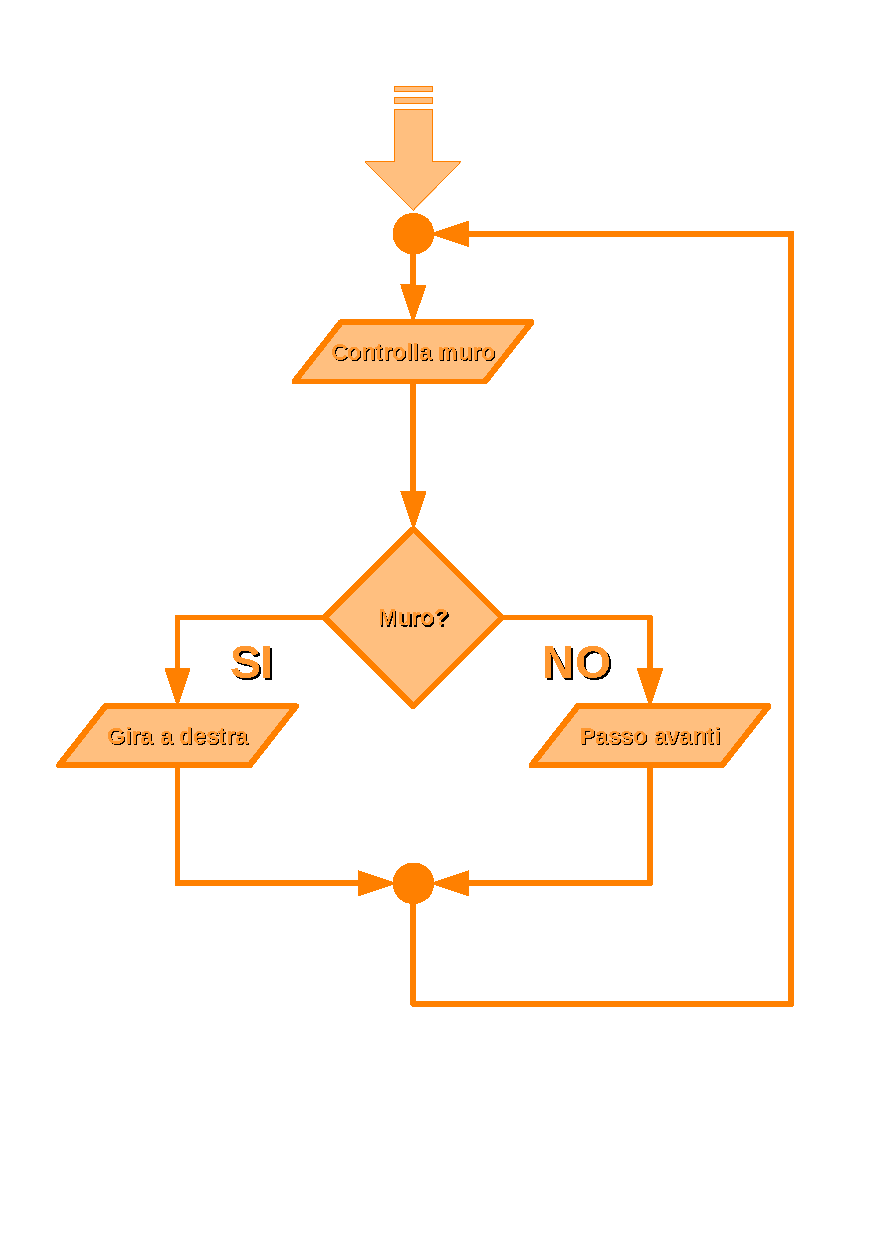
\includegraphics[scale=0.7]{Diagrams/diag1}
    				\caption{Esempio di logica di un videogioco - \textit{Come evitare gli ostacoli}.}
    			\end{figure}
    		
    			La logica serve anche a gestire situazioni diverse dal semplice \texttt{SI} e \texttt{NO}; famoso è il \textit{sillogismo}\footnote{Termine filosofico con cui Aristotele designò la forma fondamentale di argomentazione logica, costituita da tre proposizioni dichiarative connesse in modo tale che dalle prime due, assunte come premesse, si possa dedurre una conclusione. - Treccani} di Aristotele:
    			\begin{example}[Sillogismo]
    				Sillogismo di Aristotele:
    				\begin{enumerate}
    					\item Tutti gli \textbf{uomini} sono \textbf{mortali};
    					\item Socrate è \textbf{uomo};
    					\item Dunque Socrate è \textbf{mortale}.
    				\end{enumerate}
    			\end{example}
    		
				Un esempio diverso di logica è quella che può mostrare il contenuto multimediale (un video) 
				attraverso il monitor del vostro computer o la televisione a cui avete collegato la vostra consolle preferita:
    			\begin{example}[Logica: Riproduzione video]~
					\begin{itemize}
						\item L'utente ha scelto il \textsc{video}?
							\subitem \texttt{SI}
						\item Il video è pronto per essere riprodotto?
							\subitem \texttt{SI}
						\item L'utente ha premuto il tasto \textsc{play}?
							\subitem \texttt{SI}
						\item Riproduci \textsc{video} attraverso \textsc{monitor}.
					\end{itemize}
    			\end{example}
    			\begin{exercise}
    				Prova ad inventare un sillogismo.
    			\end{exercise}
    			\begin{exercise}
    				Prova a disegnare uno schema logico del sillogismo di Aristotele.
    			\end{exercise}
    		
    			La logica ci aiuta anche in altre situazioni. Quando abbiamo bisogno di \textit{prevedere} (ricordiamoci che non siamo dei maghi!) qualcosa, ad esempio:
    			\begin{example}[Previsione]Se piove o fa freddo, non esco a giocare.
    				\\Dati:\\
    				\\Fuori piove.\\Fuori fa freddo.\\
    				\\\textbf{Esco?}
    				\\\textbf{No.}
    			\end{example}
    			\begin{example}[Previsione] Se ho fame oppure è l'ora di pranzo, allora mangio.\\
    				Dati:\\
					\\Ho fame.
					\\Non è l'ora di pranzo.\\
    				\\\textbf{Mangio?}
    				\\\textbf{Si.}
    			\end{example}
    		
    			Abbiamo appena visto due esempi di \textit{previsione} conoscendo le \textit{informazioni} (negli esempi le abbiamo chiamate \textit{dati}); la differenza sostanziale con i sillogismi è molto fine ma decisiva: la condizione iniziale è \textsc{Vera} se il dato $1$ \textbf{E} il dato $2$ sono \textsc{Veri}. Nel secondo caso invece, la condizione iniziale è \textsc{Vera} se il dato $1$ \textbf{OPPURE} il dato $2$ è \textsc{Vero}.
    			
    			La logica è formata da \textbf{proposizioni} e \textbf{connettivi}, nel corso dei capitoli avremo la possibilità di dargli una definizione operativa, più intuitiva e divertente. Per ora basta sapere che c'è (ed è importante).
    		
    		\section{Gli strumenti informatici}\index{Gli strumenti informatici}
    		\label{sec: Gli strumenti informatici}
    			Cominciamo a mettere le mani in pasta!
    			In un laboratorio di informatica, oltre che leggere e studiare, si utilizza un computer. Ovviamente il computer è solo il più importante degli strumenti informatici che abbiamo al giorno d'oggi; il più importante da saper utilizzare, sul quale capire le basi dell'informatica e dell'utilizzo di questa strana tecnologia.
    			
    			Altri strumenti sono tutti quegli oggetti che possiamo utilizzare o meno nella vita di tutti i giorni, connessi la mondo dell'informatica, quali:
    			\begin{itemize}
    				\item Lo smartphone
    				\item Lo smartwatch
    				\item Il tablet
    				\item La consolle di gioco
    			\end{itemize}
    		
    			Cosa hanno in comune con il computer? Beh, proviamo a ragionare insieme: tutti hanno un'\textit{interfaccia} con voi (l'\textit{utente}), tutti ricevono dei \textit{comandi} più o meno complessi con voi, tutti \textit{computano} informazioni e ne restituiscono altre in modo diverso. Allora la domanda sorge spontanea: che differenza c'è con il classico computer?
    			
				La risposta breve e più facile è: "nulla!"
				La risposta più giusta, completa e lunga è: "sono sistemi di computazione che elaborano informazioni restituendone di altre, anche in modo diverso, e la differenza gli uni dagli altri è caratterizzata da alcune capacità presenti ed il modo più o meno efficiente di gestire alcune informazioni".\\
				
				Sento già le voci di tutti voi urlare: "Eh? Cosa? Che?"\\
				
				Tranquilli, quella di prima è solo la versione lunga della storia; in breve possiamo dire che tutti quei strumenti informatici non sono altro che computer \textbf{ottimizzati} per un determinato scopo. Secondo voi è comodo portarsi in giro la consolle di gioco oppure il computer per telefonare ad un vostro amico? È comodo portarsi in giro il tablet oppure la consolle di gioco per guardare l'orario? È comodo leggere un libro tramite la consolle?\\
				
				Eppure, tutti gli strumenti sopra elencati possono fare le stesse cose! È tutta questione di comodità.
				
				\begin{exercise}[Comodità degli strumenti informatici] Indicare quale strumento è più comodo per lo scopo:\\
					\begin{tabular}{|>{\raggedright\arraybackslash}p{5cm}|p{8cm}|}
						\hline 
						\rule[-1ex]{0pt}{5ex} Ascoltare una canzone &  \\ 
						\hline 
						\rule[-1ex]{0pt}{5ex} Videogiochi &  \\ 
						\hline 
						\rule[-1ex]{0pt}{5ex} Leggere un libro &  \\ 
						\hline 
						\rule[-1ex]{0pt}{5ex} Chiamare un amico &  \\ 
						\hline 
						\rule[-1ex]{0pt}{5ex} Leggere un messaggio &  \\ 
						\hline 
						\rule[-1ex]{0pt}{5ex} Guardare l'orario &  \\ 
						\hline 
						\rule[-1ex]{0pt}{5ex} Leggere un'email &  \\ 
						\hline 
						\rule[-1ex]{0pt}{5ex} Guardare un'immagine &  \\ 
						\hline 
					\end{tabular} 	
				\end{exercise}
    			
    			Tralasciando per ora gli altri sistemi informatici, andiamo ad analizzare lo strumento principale del laboratorio informatico: il \textbf{computer}. Ma cosa è un computer? A cosa serve? Come possiamo divertirci, studiare, lavorare con un computer?
    			Scopriamolo insieme!
    			\begin{quote}
    				\textit{"Parte della disumanità del computer sta nel fatto che, una volta programmato e messo in funzione, si comporta in maniera perfettamente onesta."}\\
    				Isaac Asimov - Chimico, scrittore.
    			\end{quote}
    		
    	\chapter{Il computer}\index{Il computer}
    	\label{cap: Il computer}
    		Cominciamo dando una bella definizione formale\footnote{Paul E. Ceruzzi - Storia dell'informatica. Dai primi computer digitali all'era di Internet}:
    		\begin{quote}
				\textit{Elaboratore o calcolatore, macchina automatizzata programmabile in grado di eseguire sia complessi calcoli matematici (calcolatore) sia altri tipi di elaborazioni dati (elaboratore).}
    		\end{quote}
    	
    		
    		
    		\section{Da cosa è formato?}\index{Da cosa è formato?}
    		\label{sec: Da cosa è formato?}
    		
    		\section{Le periferiche}\index{Le periferiche}
    		\label{sec: Le periferiche}
    		
    		\section{Il laptop}\index{Il laptop}
    		\label{sec: Il laptop}
    		
    	\chapter{Input ed output}\index{Input ed output}
    	\label{cap: Input ed output}
    		
    		\subsection{Periferiche di input}\index{Periferiche di input}
    		\label{sub: Periferiche di input}
    		
    		\subsection{Periferiche di output}\index{Periferiche di output}
    		\label{sub: Periferiche di output}
    		
    	\chapter{Usiamo il computer!}\index{Usiamo il computer!}
    	\label{cap: Usiamo il computer!}
    	%\chapter{Logica}
    		
    			
            %\lipsum[1-7] % Dummy text
        
            %------------------------------------------------
    
        \section{Citation}\index{Citation}
    
        This statement requires citation \cite{book_key}; this one is more specific \cite[122]{article_key}.
    
        %------------------------------------------------
    
    \section{Lists}\index{Lists}
    
    Lists are useful to present information in a concise and/or ordered way\footnote{Footnote example...}.
    
    \subsection{Numbered List}\index{Lists!Numbered List}
    
    \begin{enumerate}
    \item The first item
    \item The second item
    \item The third item
    \end{enumerate}
    
    \subsection{Bullet Points}\index{Lists!Bullet Points}
    
    \begin{itemize}
    \item The first item
    \item The second item
    \item The third item
    \end{itemize}
    
    \subsection{Descriptions and Definitions}\index{Lists!Descriptions and Definitions}
    
    \begin{description}
    \item[Name] Description
    \item[Word] Definition
    \item[Comment] Elaboration
    \end{description}
    
    %----------------------------------------------------------------------------------------
    %	CHAPTER 2
    %----------------------------------------------------------------------------------------
    
    \chapter{In-text Elements}
    
    \section{Theorems}\index{Theorems}
    
    This is an example of theorems.
    
    \subsection{Several equations}\index{Theorems!Several Equations}
    This is a theorem consisting of several equations.
    
    \begin{theorem}[Name of the theorem]
    In $E=\mathbb{R}^n$ all norms are equivalent. It has the properties:
    \begin{align}
    & \big| ||\mathbf{x}|| - ||\mathbf{y}|| \big|\leq || \mathbf{x}- \mathbf{y}||\\
    &  ||\sum_{i=1}^n\mathbf{x}_i||\leq \sum_{i=1}^n||\mathbf{x}_i||\quad\text{where $n$ is a finite integer}
    \end{align}
    \end{theorem}
    
    \subsection{Single Line}\index{Theorems!Single Line}
    This is a theorem consisting of just one line.
    
    \begin{theorem}
    A set $\mathcal{D}(G)$ in dense in $L^2(G)$, $|\cdot|_0$. 
    \end{theorem}
    
    %------------------------------------------------
    
    \section{Definitions}\index{Definitions}
    
    This is an example of a definition. A definition could be mathematical or it could define a concept.
    
    \begin{definition}[Definition name]
    Given a vector space $E$, a norm on $E$ is an application, denoted $||\cdot||$, $E$ in $\mathbb{R}^+=[0,+\infty[$ such that:
    \begin{align}
    & ||\mathbf{x}||=0\ \Rightarrow\ \mathbf{x}=\mathbf{0}\\
    & ||\lambda \mathbf{x}||=|\lambda|\cdot ||\mathbf{x}||\\
    & ||\mathbf{x}+\mathbf{y}||\leq ||\mathbf{x}||+||\mathbf{y}||
    \end{align}
    \end{definition}
    
    %------------------------------------------------
    
    \section{Notations}\index{Notations}
    
    \begin{notation}
    Given an open subset $G$ of $\mathbb{R}^n$, the set of functions $\varphi$ are:
    \begin{enumerate}
    \item Bounded support $G$;
    \item Infinitely differentiable;
    \end{enumerate}
    a vector space is denoted by $\mathcal{D}(G)$. 
    \end{notation}
    
    %------------------------------------------------
    
    \section{Remarks}\index{Remarks}
    
    This is an example of a remark.
    
    \begin{remark}
    The concepts presented here are now in conventional employment in mathematics. Vector spaces are taken over the field $\mathbb{K}=\mathbb{R}$, however, established properties are easily extended to $\mathbb{K}=\mathbb{C}$.
    \end{remark}
    
    %------------------------------------------------
    
    \section{Corollaries}\index{Corollaries}
    
    This is an example of a corollary.
    
    \begin{corollary}[Corollary name]
    The concepts presented here are now in conventional employment in mathematics. Vector spaces are taken over the field $\mathbb{K}=\mathbb{R}$, however, established properties are easily extended to $\mathbb{K}=\mathbb{C}$.
    \end{corollary}
    
    %------------------------------------------------
    
    \section{Propositions}\index{Propositions}
    
    This is an example of propositions.
    
    \subsection{Several equations}\index{Propositions!Several Equations}
    
    \begin{proposition}[Proposition name]
    It has the properties:
    \begin{align}
    & \big| ||\mathbf{x}|| - ||\mathbf{y}|| \big|\leq || \mathbf{x}- \mathbf{y}||\\
    &  ||\sum_{i=1}^n\mathbf{x}_i||\leq \sum_{i=1}^n||\mathbf{x}_i||\quad\text{where $n$ is a finite integer}
    \end{align}
    \end{proposition}
    
    \subsection{Single Line}\index{Propositions!Single Line}
    
    \begin{proposition} 
    Let $f,g\in L^2(G)$; if $\forall \varphi\in\mathcal{D}(G)$, $(f,\varphi)_0=(g,\varphi)_0$ then $f = g$. 
    \end{proposition}
    
    %------------------------------------------------
    
    \section{Examples}\index{Examples}
    
    This is an example of examples.
    
    \subsection{Equation and Text}\index{Examples!Equation and Text}
    
    \begin{example}
    Let $G=\{x\in\mathbb{R}^2:|x|<3\}$ and denoted by: $x^0=(1,1)$; consider the function:
    \begin{equation}
    f(x)=\left\{\begin{aligned} & \mathrm{e}^{|x|} & & \text{si $|x-x^0|\leq 1/2$}\\
    & 0 & & \text{si $|x-x^0|> 1/2$}\end{aligned}\right.
    \end{equation}
    The function $f$ has bounded support, we can take $A=\{x\in\mathbb{R}^2:|x-x^0|\leq 1/2+\epsilon\}$ for all $\epsilon\in\intoo{0}{5/2-\sqrt{2}}$.
    \end{example}
    
    \subsection{Paragraph of Text}\index{Examples!Paragraph of Text}
    
    \begin{example}[Example name]
    \lipsum[2]
    \end{example}
    
    %------------------------------------------------
    
    \section{Exercises}\index{Exercises}
    
    This is an example of an exercise.
    
    \begin{exercise}
    This is a good place to ask a question to test learning progress or further cement ideas into students' minds.
    \end{exercise}
    
    %------------------------------------------------
    
    \section{Problems}\index{Problems}
    
    \begin{problem}
    What is the average airspeed velocity of an unladen swallow?
    \end{problem}
    
    %------------------------------------------------
    
    \section{Vocabulary}\index{Vocabulary}
    
    Define a word to improve a students' vocabulary.
    
    \begin{vocabulary}[Word]
    Definition of word.
    \end{vocabulary}
    
    %----------------------------------------------------------------------------------------
    %	PART
    %----------------------------------------------------------------------------------------
    
    \part{Part Two}
    
    %----------------------------------------------------------------------------------------
    %	CHAPTER 3
    %----------------------------------------------------------------------------------------
    
    \chapterimage{chapter_head_1.pdf} % Chapter heading image
    
    \chapter{Presenting Information}
    
    \section{Table}\index{Table}
    
    \begin{table}[h]
    \centering
    \begin{tabular}{l l l}
    \toprule
    \textbf{Treatments} & \textbf{Response 1} & \textbf{Response 2}\\
    \midrule
    Treatment 1 & 0.0003262 & 0.562 \\
    Treatment 2 & 0.0015681 & 0.910 \\
    Treatment 3 & 0.0009271 & 0.296 \\
    \bottomrule
    \end{tabular}
    \caption{Table caption}
    \end{table}
    
    %------------------------------------------------
    
    \section{Figure}\index{Figure}
    
    \begin{figure}[h]
    \centering
\includegraphics[scale=0.5]{placeholder}
    \caption{Figure caption}
    \end{figure}
    
    %----------------------------------------------------------------------------------------
    %	BIBLIOGRAPHY
    %----------------------------------------------------------------------------------------
    
    \chapter*{Bibliography}
    \addcontentsline{toc}{chapter}{\textcolor{ocre}{Bibliography}}
    \section*{Books}
    \addcontentsline{toc}{section}{Books}
    \printbibliography[heading=bibempty,type=book]
    \section*{Articles}
    \addcontentsline{toc}{section}{Articles}
    \printbibliography[heading=bibempty,type=article]
    
    %----------------------------------------------------------------------------------------
    %	INDEX
    %----------------------------------------------------------------------------------------
    
    \cleardoublepage
    \phantomsection
    \setlength{\columnsep}{0.75cm}
    \addcontentsline{toc}{chapter}{\textcolor{ocre}{Index}}
    \printindex
    
    %----------------------------------------------------------------------------------------

\end{document}
